% =====================================================================================
%  SI.tex — Supplementary Material, ported from sections/SI.md (v10, APPROVED 2026-09-18).
%  Standalone document (separate from the main paper). Sections S1–S6.
%  Floats: Tables S1–S6, Figures S1–S9.
%
%  Cross-references to the main text are written out in words ("Sec. II A of the main
%  text") because this is a separate document; if the two are merged, convert them to
%  \ref{} against the main paper's labels.
% =====================================================================================
\documentclass[10pt]{article}
\usepackage[margin=1in]{geometry}
\usepackage{amsmath,amssymb}
\usepackage{booktabs}
\usepackage{graphicx}
\usepackage{siunitx}
\usepackage{hyperref}
\usepackage[numbers,sort&compress]{natbib}

\graphicspath{{figures/}}

\newcommand{\dZ}{\ensuremath{\Delta Z}}
\newcommand{\dEN}{\ensuremath{\Delta E/N}}
\newcommand{\eVA}{\ensuremath{\text{eV/atom}}}

\renewcommand{\thesection}{S\arabic{section}}
\renewcommand{\thetable}{S\arabic{table}}
\renewcommand{\thefigure}{S\arabic{figure}}
\setcounter{secnumdepth}{3}
\renewcommand{\thesubsubsection}{\thesection.\arabic{subsubsection}}
\setlength{\emergencystretch}{2em}

\title{Supplementary Material:\\ Effect of boron insertion on metal-film wetting of Fe on MgO}
\author{Andi Muhammad Nur Fitrah Syamsul\thanks{Graduate School of Engineering, Mie University,
Tsu, Mie 514-8507, Japan.}\and Kohji Nakamura}
\date{\today}

\begin{document}
\maketitle

\section{Performance of the biased exploration in finding the global minimum}
\label{sec:S1}

The main text uses only structures from iteration $\ge 10$, because relaxation of candidates begins
at that iteration. Here we instead use all iterations of the Fe/MgO model---the model with
the largest number of independent searches (13)---to characterise how the biased exploration
progresses towards the global minimum, and to show what the discarded early iterations contain.
Energies are given as $\dEN = (E - E_\text{globalmin})/N$ relative to the lowest energy found
anywhere in the 13 searches, so the best-known energy descends to zero (Fig.~\ref{fig:S1}).

\begin{figure}[t]
\centering
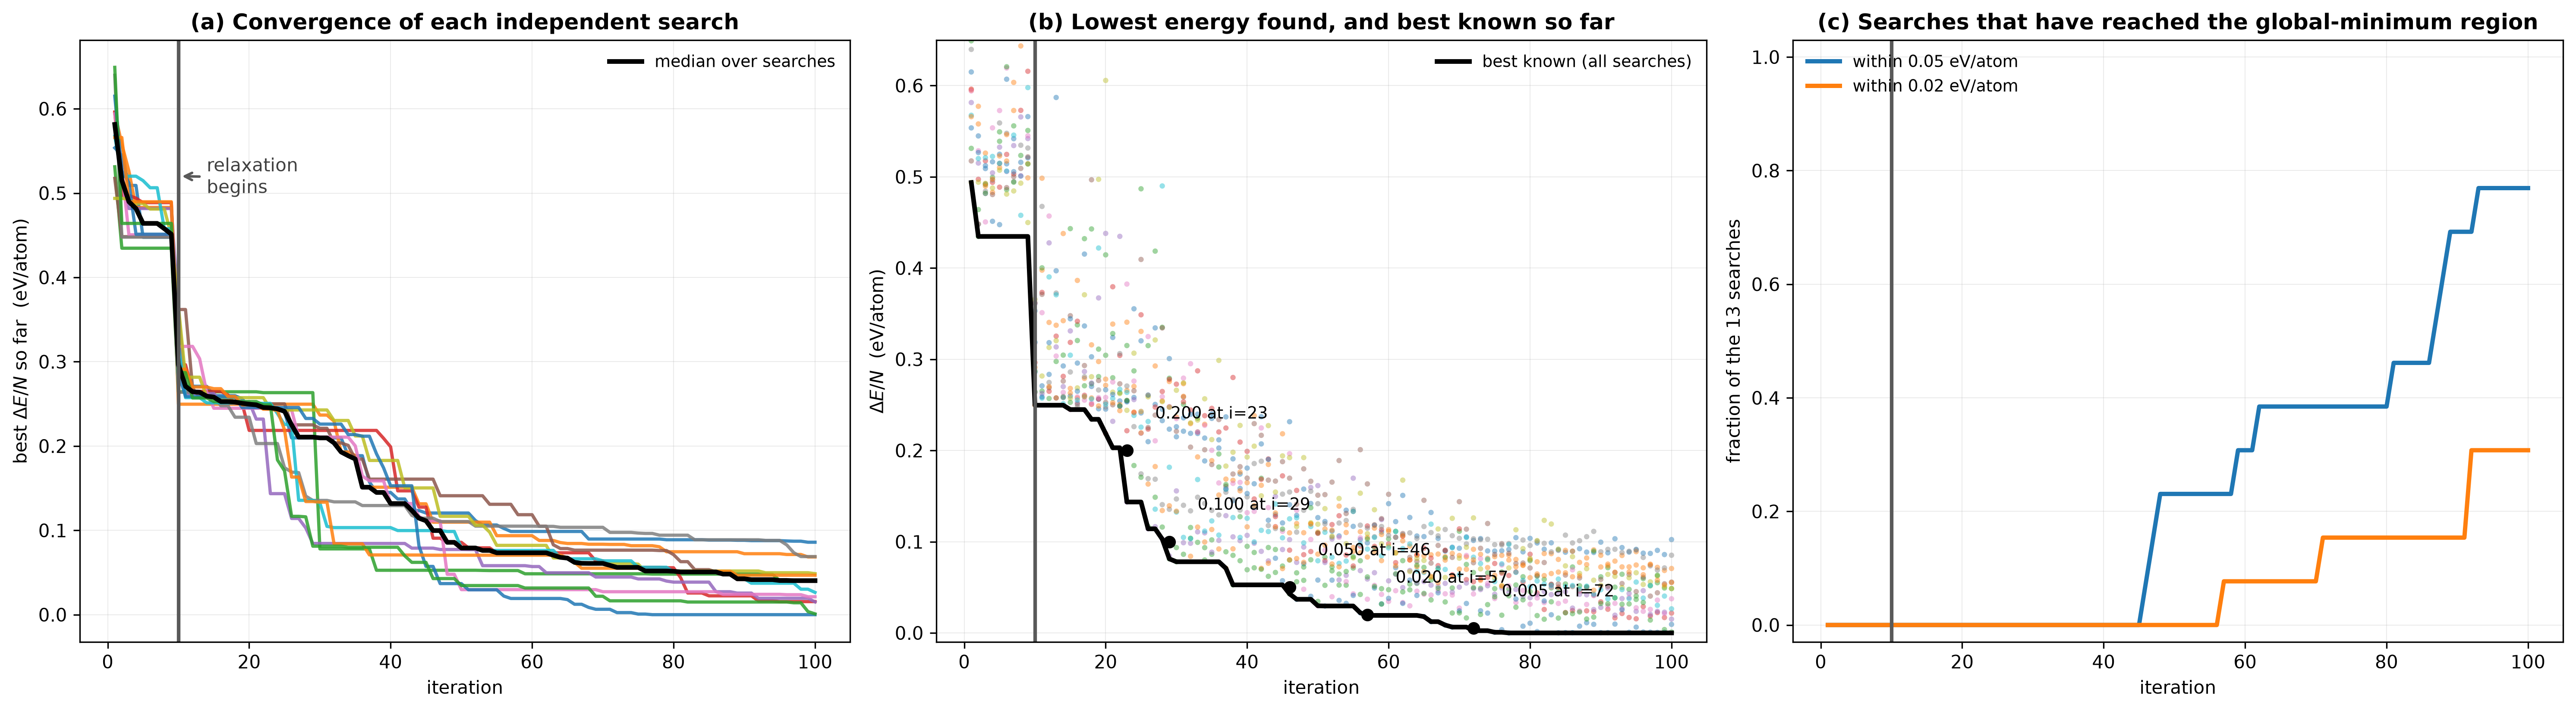
\includegraphics[width=\textwidth]{exploration_performance_femgo.png}
\caption{\label{fig:S1}Best-so-far $\Delta E/N$ against iteration for each of the 13 searches, with
the median over searches in black; (b) the lowest energy found in each iteration (points) and the
best-known energy across all searches (black line), with the iterations at which it first crosses
0.20, 0.10, 0.05, 0.02 and 0.005~\eVA{} marked; (c) the fraction of searches whose own best-so-far
has come within 0.05 and 0.02~\eVA{} of the global minimum. The vertical line in each panel marks
iteration 10, where relaxation begins.}
\end{figure}

\subsubsection{The onset of relaxation is the pivot of the search} Across iterations 1--9 the best-known
energy falls only from 0.494 to 0.435~\eVA---0.06~\eVA, about 12\,\% of the total descent of the run.
At iteration 10, the first iteration at which candidates are surrogate-relaxed, it drops from 0.435
to 0.250~\eVA{} in a single iteration: approximately half of the entire descent of the run
(49\,\%) occurs at the onset of relaxation. The per-search drop across the onset has a median of
0.165~\eVA{} and a range of 0.084--0.233~\eVA, so the step is a property of every search rather than
of one.

\subsubsection{Before the onset the candidates cannot be ranked} The structures evaluated in iterations
1--9 are unrelaxed placements, so their energy ordering reflects the starting geometry rather than
any relaxed configuration: several searches plateau after the second or third iteration and show no
further improvement for the remainder of the pre-relaxation phase. This is why the main-text analysis
discards them, and why their exclusion is not a loss of evidence.

\subsubsection{After the onset the descent proceeds in a long, progressively finer sequence} The
best-known energy reaches 0.219 ($i = 20$), 0.078 ($i = 30$) and 0.030~\eVA{} ($i = 50$)---84\,\% of
the total descent complete by iteration 30 and 94\,\% by iteration 50---with successive crossings of
0.20~\eVA{} at $i = 23$, 0.10 at $i = 29$, 0.05 at $i = 46$, 0.02 at $i = 57$ and 0.005 at $i = 72$.
The global minimum is first reached at iteration 77 by one of the searches, and the searches are
still making small improvements when the run ends at iteration 100.

\subsubsection{The searches do not agree on the answer} Only 10 of the 13 searches end within 0.05~\eVA{}
of the global minimum, and only 4 within 0.02; the median search finishes 0.040~\eVA{} above it
(per-search final values 0.000--0.086~\eVA). A single search supplies the global minimum and a second
comes within 0.001~\eVA{} of it. The final energy reached by a search therefore carries a sizeable
spread, which is why the main text compares basins across searches rather than quoting one structure
per model.

\section{Electronic-structure origin of the flat $\to$ island transition}
\label{sec:S2}

Section IV A of the main text attributes the island ground state to the loss of forced interfacial
coupling. Here we test that reading directly, by comparing the flat reference monolayer
($\dZ = 0.000$~\AA) with the island ground state ($\dZ = 3.652$~\AA) of the Fe/MgO model in
the \emph{same} projection set, so the two are directly comparable (GPAW, linear combination of
atomic orbitals (LCAO) with a double-zeta polarised basis, the Perdew--Burke--Ernzerhof (PBE)
functional, kpts $(12,12,1)$, 2000 points, width 0.15~eV, Fermi-shifted). Projections are per atom: Fe-$d_{z^2}$
($l = 2$, $m = 2$) and O-$p_z$ ($l = 1$, $m = 0$). $d$-band moments are taken over $[-5, +3]$~eV
around $E_F$. All numbers in this section are those of Table~\ref{tab:S1} and Table~\ref{tab:S2}.

\begin{figure}[t]
\centering
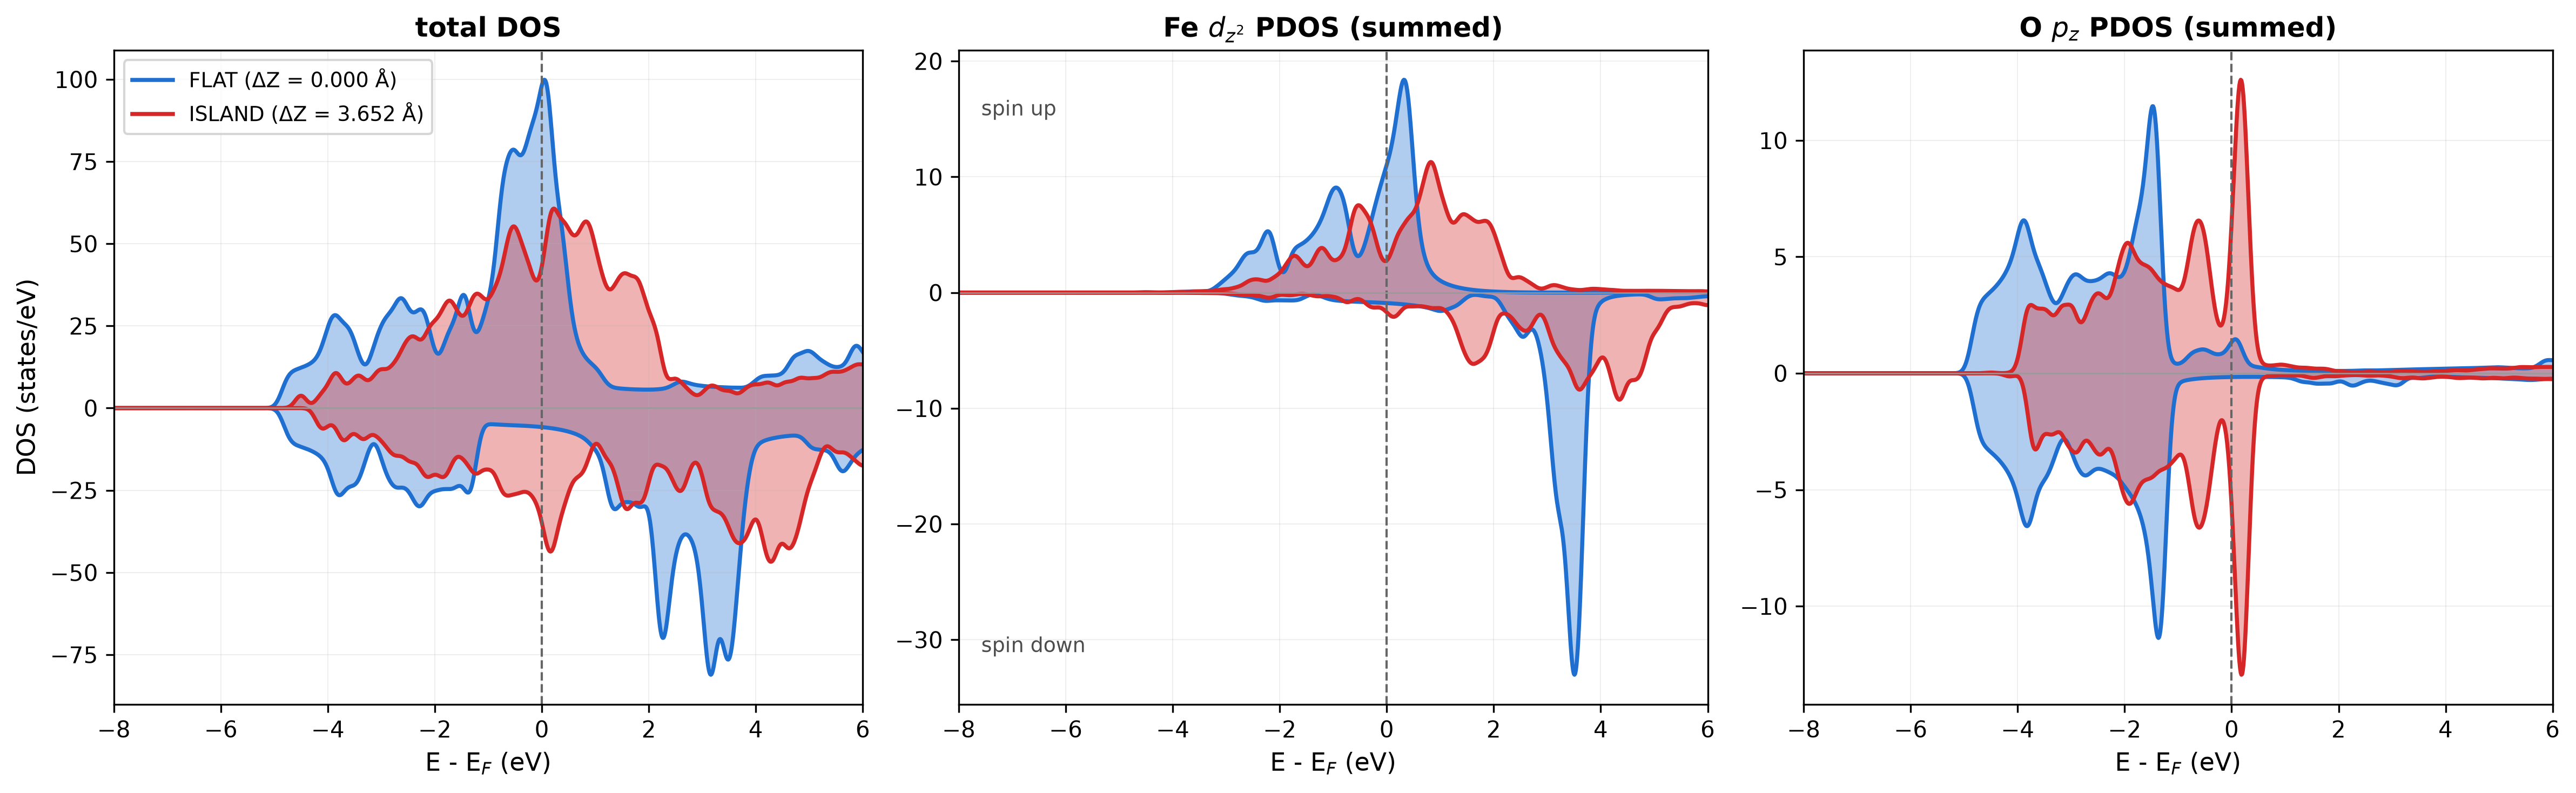
\includegraphics[width=\textwidth]{pdos_flat_vs_island.png}
\caption{\label{fig:S2}Total density of states (DOS), Fe-$d_{z^2}$ and O-$p_z$ for the flat monolayer (blue) and the
island ground state (red).}
\end{figure}

\begin{table}[t]
\small
\caption{\label{tab:S1}Density-of-states metrics for the two configurations. \emph{[SI-1, SI-2]}}
\begin{tabular*}{\textwidth}{@{\extracolsep{\fill}}lccc}
\toprule
Quantity & Flat & Island & $\Delta$ (island $-$ flat) \\
\midrule
$d$-band centre (eV) & $-0.2294$ & $+0.6013$ & $+0.83$ (up) \\
$d$-band width (eV)  & $1.4171$  & $1.3139$  & $-0.10$ (narrower) \\
Fe-$d_{z^2}$ integral & $31.7136$ & $33.8763$ & $+2.16$ (more filled) \\
O-$p_z$ integral      & $43.8799$ & $42.3738$ & $-1.51$ ($-3.4$\,\%) \\
Spin polarisation     & $5.8050$  & $4.3695$  & $-1.44$ (less magnetic) \\
DOS at $E_F$          & $103.9621$ & $78.0885$ & $-25.9$ ($-25$\,\%) \\
\bottomrule
\end{tabular*}
\end{table}

\subsubsection{Islanding reduces Fe--O hybridisation} \emph{[SI-1]} Going flat $\to$ island, the Fe
$d$-band centre rises by +0.83~eV while the O-$p_z$ integral falls by 3.4\,\% and the
Fe-$d_{z^2}$ manifold becomes slightly narrower ($-0.10$~eV) and more filled ($+2.16$). The flat
monolayer is therefore the more strongly Fe--O hybridised of the two: it mixes more O-$p$ character
and its Fe $d$-states sit lower, whereas the island's $d$-states shift up and localise.

\subsubsection{Islanding weakens the magnetic and electronic activity at $E_F$} \emph{[SI-2]} The spin
polarisation falls from 5.81 to 4.37 and the DOS at the Fermi level drops by 25\,\% (104.0 $\to$
78.1). The flat monolayer is the electronically ``hotter'' configuration; the island is quieter.

\subsubsection{Defining the interface by geometry, not by height} The island is a buckled cluster rather
than a stack of layers, so its interface cannot be defined by a height criterion: a $z$-based layer
split would cut through the cluster and misassign atoms as a function of its buckling. We therefore
define the interface geometrically: interface Fe $:=$ Fe with a nearest O within
2.8~\AA, i.e.\ Fe actually in contact with the oxide. By this criterion the flat monolayer is 25/25
interface atoms and the island only 9/25.

\begin{figure}[t]
\centering
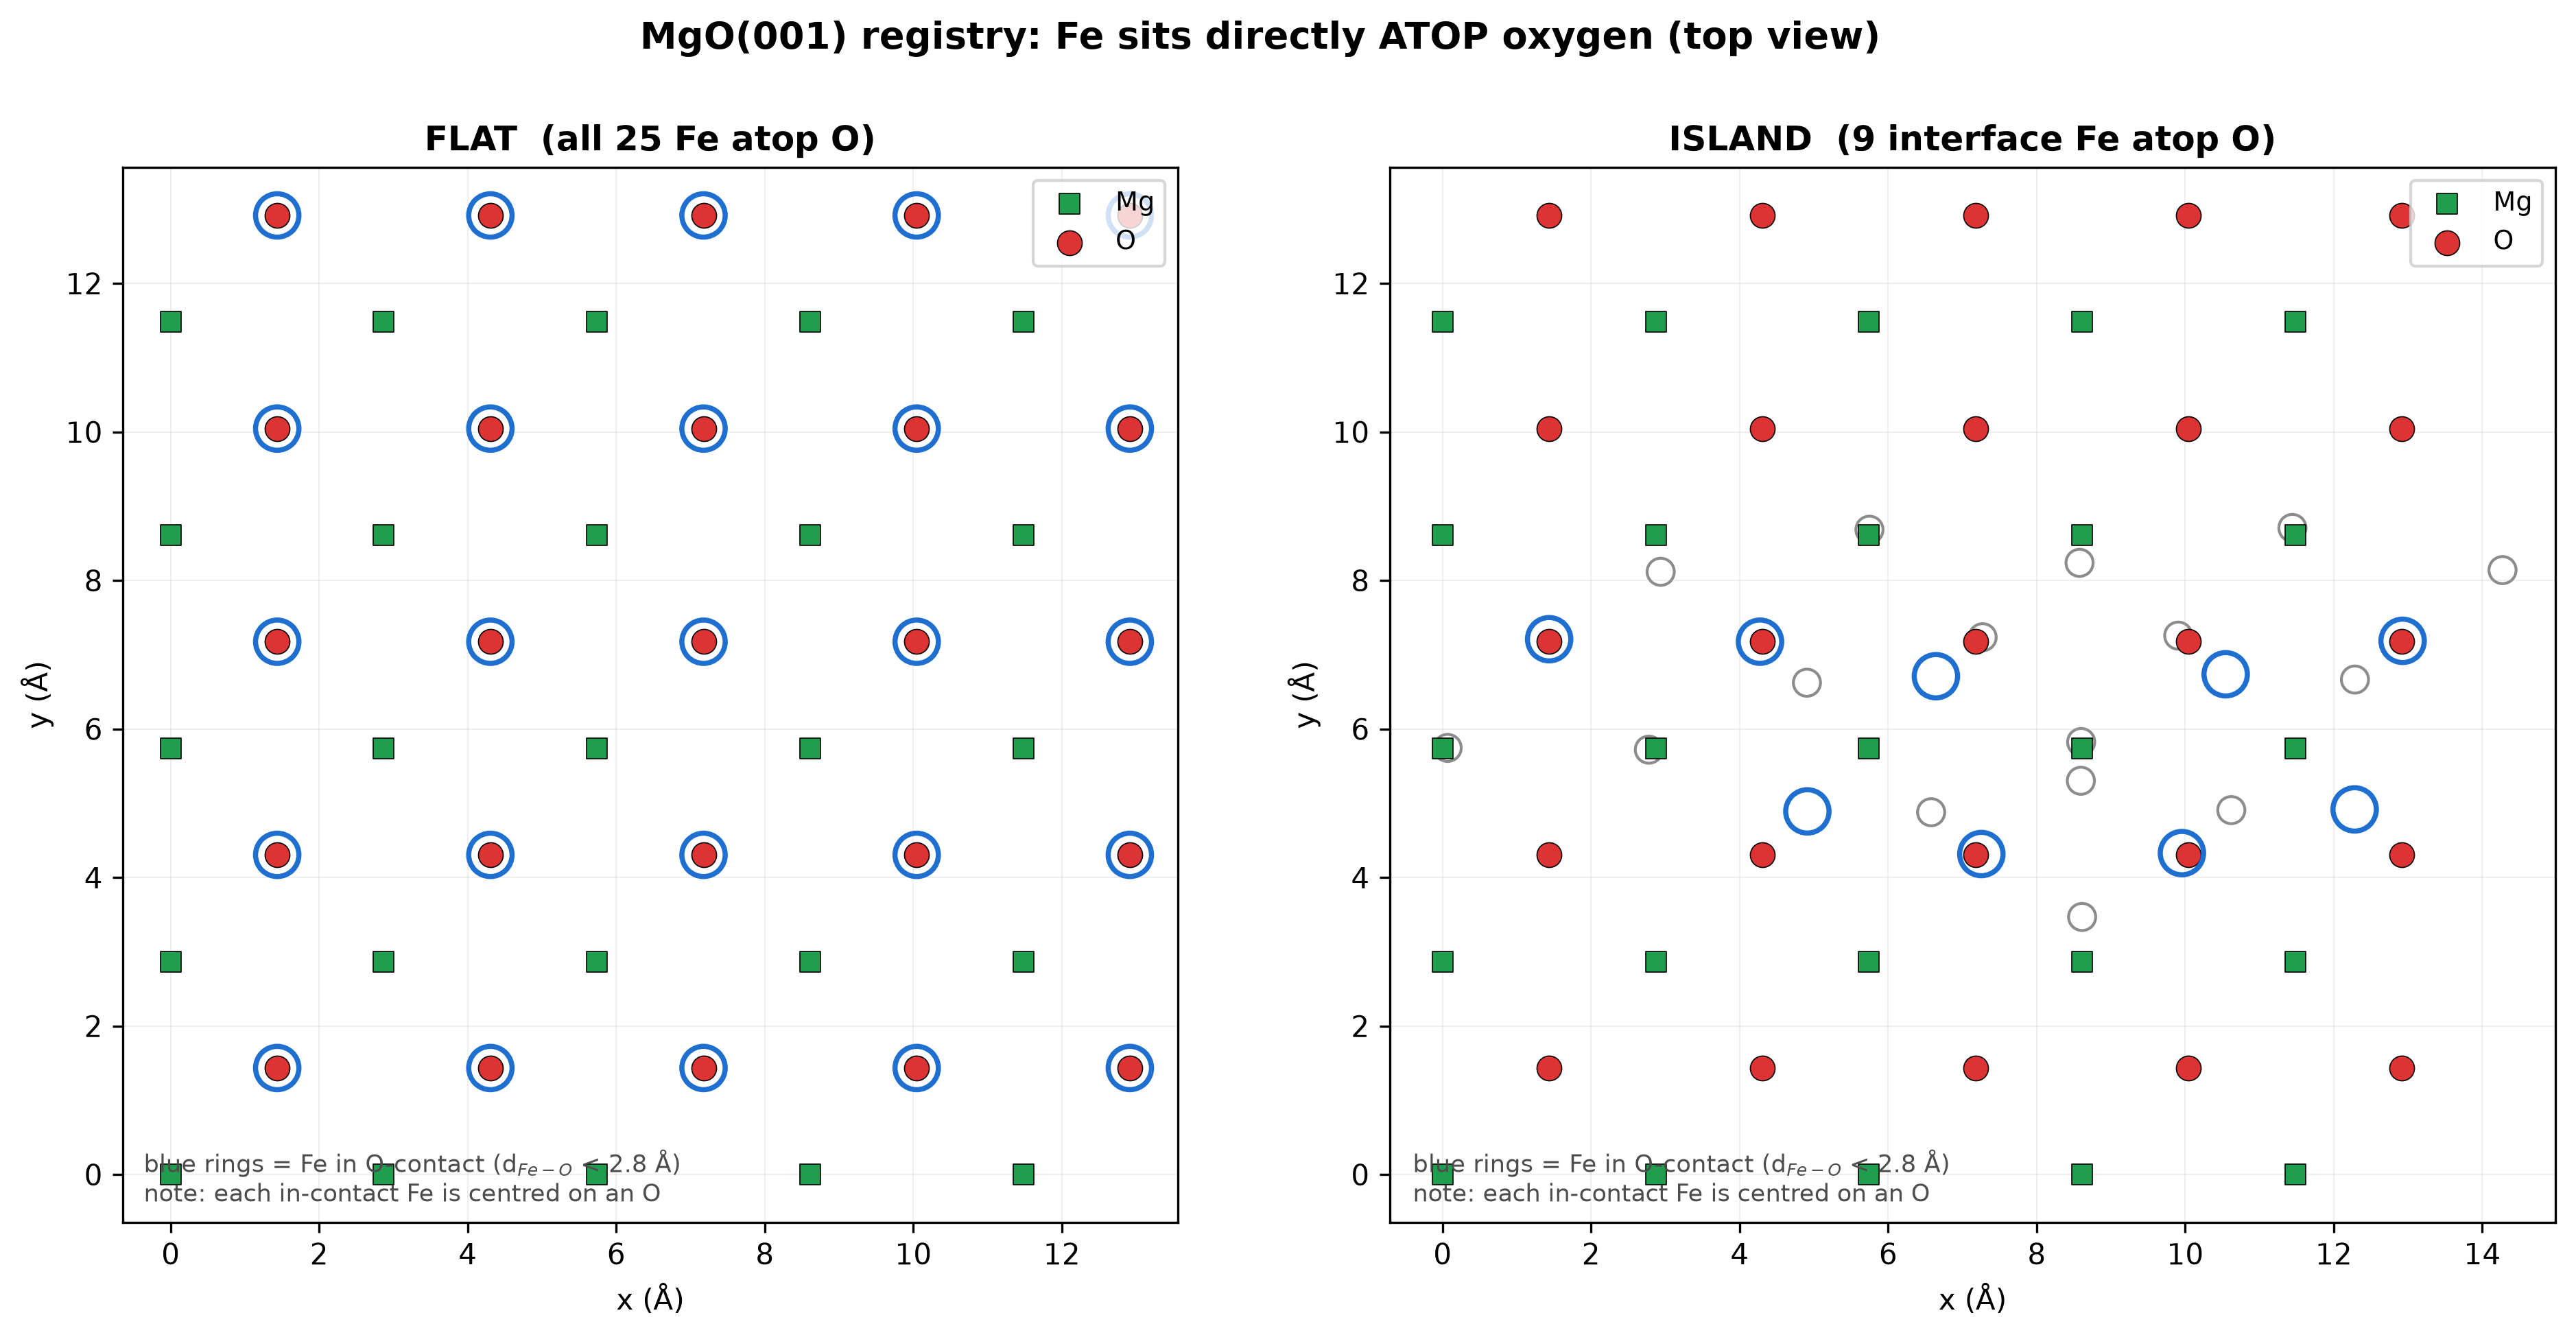
\includegraphics[width=\textwidth]{interface_registry_topview.png}
\caption{\label{fig:S3}Top view of the interface, showing the metal atoms registered directly above
the substrate oxygen on the MgO(001) lattice.}
\end{figure}

\begin{table}[t]
\footnotesize
\caption{\label{tab:S2}Site-resolved $d$-band metrics and the Fe-on-O registry, by geometric group.
The last two columns are the mean nearest-O distance and the mean in-plane offset from the
nearest substrate atom (0 $=$ directly atop); for groups that include non-contacting Fe these are not
bond lengths. \emph{[SI-3, SI-4]}}
\begin{tabular*}{\textwidth}{@{\extracolsep{\fill}}llcccccc}
\toprule
Structure & Group & $n$ & $d$-centre (eV) & width (eV) & $\int$ & $\langle$nearest $d_\mathrm{Fe-O}\rangle$ (\AA) & $\langle$offset$\rangle$ (\AA) \\
\midrule
Flat   & interface ($=$ all)          & 25 & $-0.2294$ & 1.4171 & 31.7136 & 2.3000 & 0.0000 \\
Island & interface ($d_\mathrm{Fe-O} < 2.8$~\AA) & 9 & $+0.5106$ & 1.5165 & 12.2134 & 2.3311 & 0.3722 \\
Island & non-interface                & 16 & $+0.6524$ & 1.1815 & 21.6629 & 4.3462 & 0.4726 \\
Island & all                          & 25 & $+0.6013$ & 1.3139 & 33.8763 & 3.6208 & 0.4365 \\
\bottomrule
\end{tabular*}
\end{table}

\subsubsection{The island's true interface Fe are not flat-like} \emph{[SI-3]} Restricting the comparison
to the 9 Fe atoms genuinely in O contact does not recover the flat signature: their $d$-band centre
is +0.5106~eV, against $-0.2294$~eV for the flat monolayer---a difference of 0.74~eV, larger
than the spread between the island's interface ($+0.5106$) and non-interface ($+0.6524$) groups. Two
features of the model matter here. First, the two groups sit at essentially the same
nearest-O distance (2.3311~\AA{} island vs 2.3000~\AA{} flat), and that distance is the one set when
the reference film is built---a 2.3~\AA{} interfacial separation that relaxation preserves (Sec.~II C
of the main text)---rather than an emergent quantity, so the electronic difference cannot be
a per-bond-length effect. Second, the flat layer's registry is perfect (offset 0.0000~\AA) and
uniform, whereas the island's 9 contacts are buckled (offset 0.3722~\AA) and only a third of the
film. The flat monolayer's strong Fe--O coupling is therefore a collective property of all
25 metal atoms being registry-locked in one plane, not a property of an individual Fe--O bond.

\subsubsection{The Fe-atop-O registry is a consistency check} \emph{[SI-4]} Every in-contact Fe sits
directly atop an oxygen---25/25 in the flat monolayer and 9/9 in the island---and none atop
Mg. This is the registry determined experimentally for the first monolayer of Fe on MgO(001) by
low-energy electron diffraction (LEED) I--V analysis \cite{urano1988} and used in first-principles models of the Fe$|$MgO$|$Fe interface
\cite{butler2001}, and it is also the registry the reference layer is built with---the construction
places the substrate oxygen directly above the metal sites---so the flat film's registry follows from
the construction as much as from the physics. It is reported here as a consistency check, not
as a prediction of the search. What the search does add is the island's behaviour: the Fe that
remain in contact keep O as their nearest in-plane neighbour (9/9) rather than switching to Mg, so
the island reduces the \emph{number} of Fe--O contacts (25 $\to$ 9) without abandoning their
character.

\subsubsection{Combined picture} The flat monolayer maximises Fe--O coupling by locking every metal atom
into one registered plane, at the cost of the three-dimensional Fe--Fe coordination available to a
cluster; the island reverses that trade, retaining strong individual Fe--O bonds for the third of its
atoms that remain in contact while restoring metal cohesion for the rest. This is the mechanism
stated in Sec.~IV A of the main text as reduced forced interfacial coupling plus restored
metal cohesion. It is explicitly not a lattice-strain effect: the in-plane mismatch of this
interface is carried by the substrate, which is held fixed, and the metal film sits at its own
equilibrium lattice constant (Sec.~II A and IV D of the main text).

\section{Method-parameter sensitivity of the biased exploration}
\label{sec:S3}

The search used here is a custom, biased scheme---global optimisation with first-principles energy
expressions (GOFEE), a Gaussian-process regression (GPR) surrogate with a lower confidence bound
(LCB) acquisition function, seeded from a flat Fe reference layer, with a heterostructure-aware
randomiser and a rattle generator supplying the perturbation. Here we vary three method parameters on the same
Fe$_{25}$Mg$_{25}$O$_{25}$ system and ask whether the method's conclusions survive the choice: is the
island still the ground state, how far does a single search reach, and is the flat/island basin
picture preserved. The baseline for every family is the plain Fe/MgO run (rattle 1.5/2.3,
$\kappa = 2$, no dipole correction). Energies are per-seed best $\Delta E/N$ relative to the lowest
energy found in any of these runs, $-436.909$~eV.

\subsubsection{Only completed searches are used} Several of the searches in this study were stopped
early, and they are excluded everywhere in this paper. A short search has had less time to descend,
so its per-seed best is systematically worse---every such search in this set is a severe outlier
(0.23--0.35~\eVA, against $\sim$0.03--0.09 for completed searches)---and because searches that
stopped early are not distributed evenly across the settings they would distort the comparison
between them. The same criterion is applied without exception throughout the analysis, and it is
decided from the iteration count recorded for each search, not from how a search is
labelled: a search that looks complete can have stopped early. The baseline quoted in
Table~\ref{tab:S3} therefore consists of 13 completed searches---one further search of that
family stopped early---which is the replica count used in the main text.

\begin{table}[t]
\footnotesize
\caption{\label{tab:S3}Method-parameter sensitivity; completed searches only (100 iterations).
\emph{[SI-5, SI-6, SI-7]}}
\begin{tabular*}{\textwidth}{@{\extracolsep{\fill}}llccccc}
\toprule
Family & Setting & Searches & per-seed best (\eVA) & Flat fraction & Diversity \\
\midrule
rattle & baseline (1.5 / 2.3)  & 13 & \textbf{0.03683 $\pm$ 0.02575} & 0.165 & 2.22 \\
rattle & reduced-0.5 (1.0 / 1.8) & 2 & \textbf{0.26073 $\pm$ 0.06804} & 0.023 & 3.74 \\
rattle & reduced-1.0 (0.5 / 1.3) & 4 & \textbf{0.25583 $\pm$ 0.13287} & 0.017 & 4.33 \\
kappa  & $\kappa = 2$ (baseline) & 13 & 0.03683 $\pm$ 0.02575 & 0.165 & 2.22 \\
kappa  & $\kappa = 1$            & 16 & 0.03947 $\pm$ 0.02371 & 0.182 & 2.36 \\
kappa  & $\kappa = 3$            & 10 & 0.03509 $\pm$ 0.02182 & 0.149 & 2.65 \\
kappa  & $\kappa = 4$            &  9 & 0.03209 $\pm$ 0.01872 & 0.132 & 2.68 \\
dipole & no dipole (baseline)   & 13 & 0.03683 $\pm$ 0.02575 & 0.165 & 2.22 \\
dipole & dipole $xy$            & 11 & 0.03770 $\pm$ 0.02436 & 0.158 & 2.67 \\
\bottomrule
\end{tabular*}
\end{table}

\begin{figure}[t]
\centering
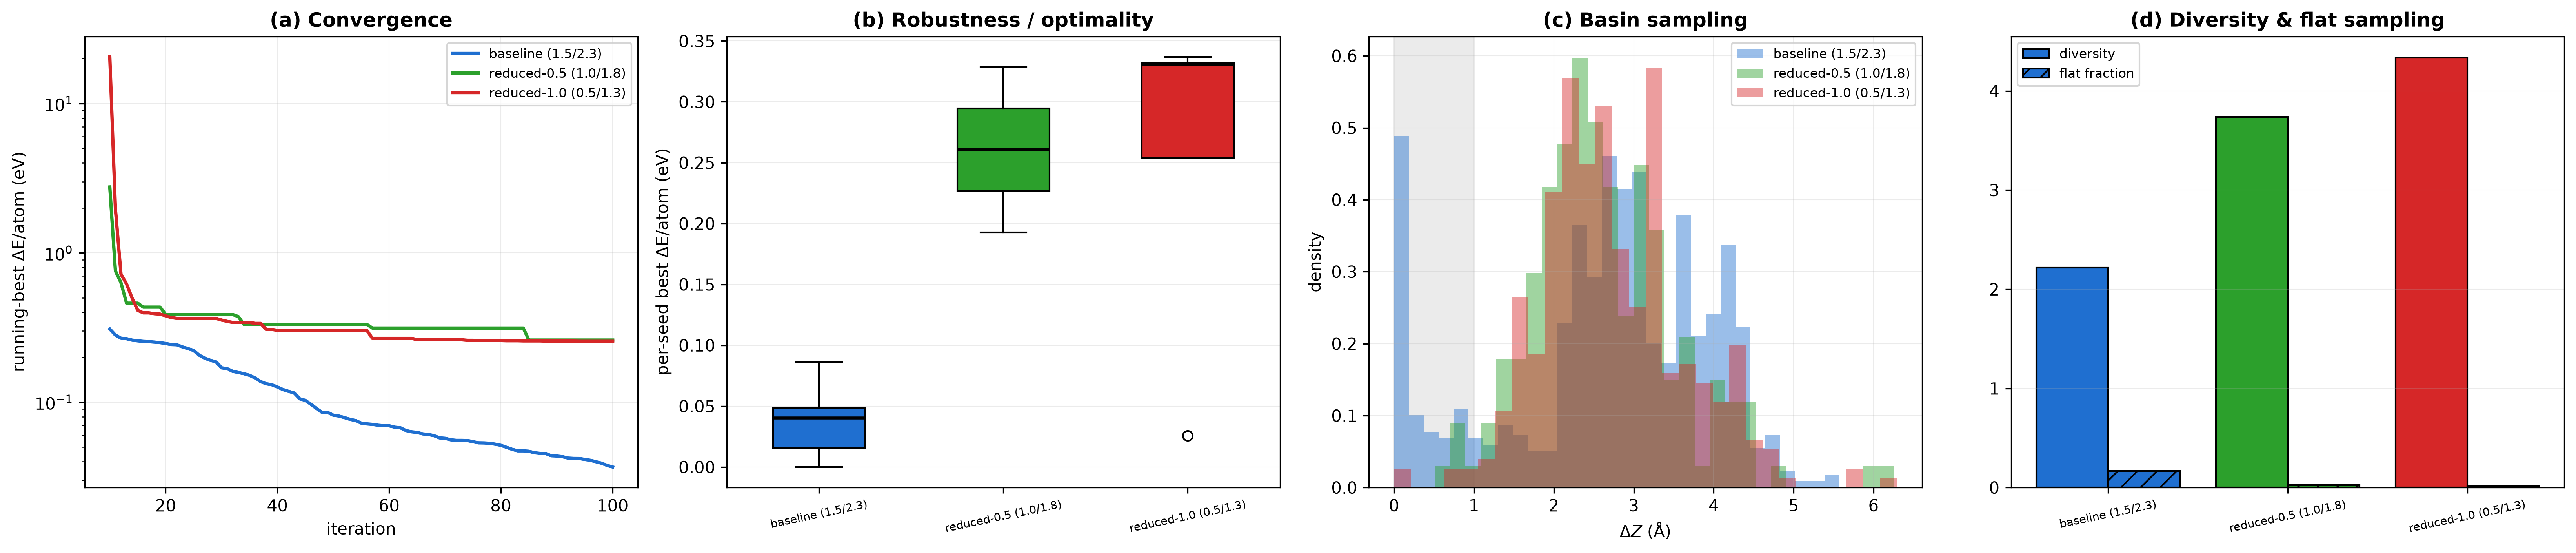
\includegraphics[width=\textwidth]{method_sensitivity_rattle.png}
\caption{\label{fig:S4}Convergence, per-seed best, basin sampling and diversity for the
rattle-strength family (four panels).}
\end{figure}

\begin{figure}[t]
\centering
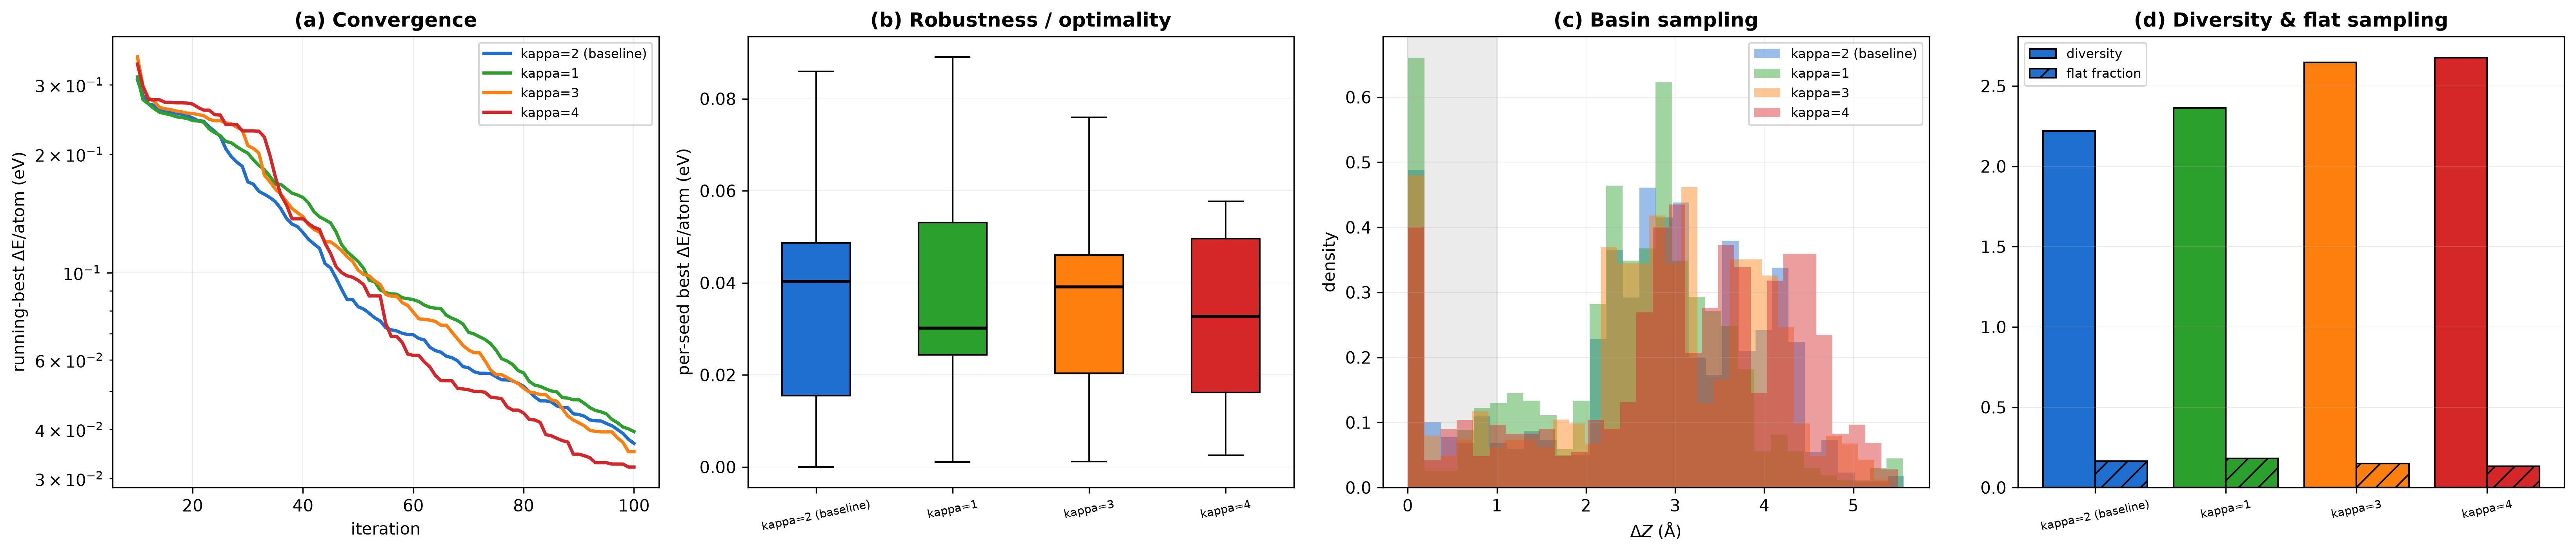
\includegraphics[width=\textwidth]{method_sensitivity_kappa.png}
\caption{\label{fig:S5}The same four panels for the kappa family.}
\end{figure}

\begin{figure}[t]
\centering
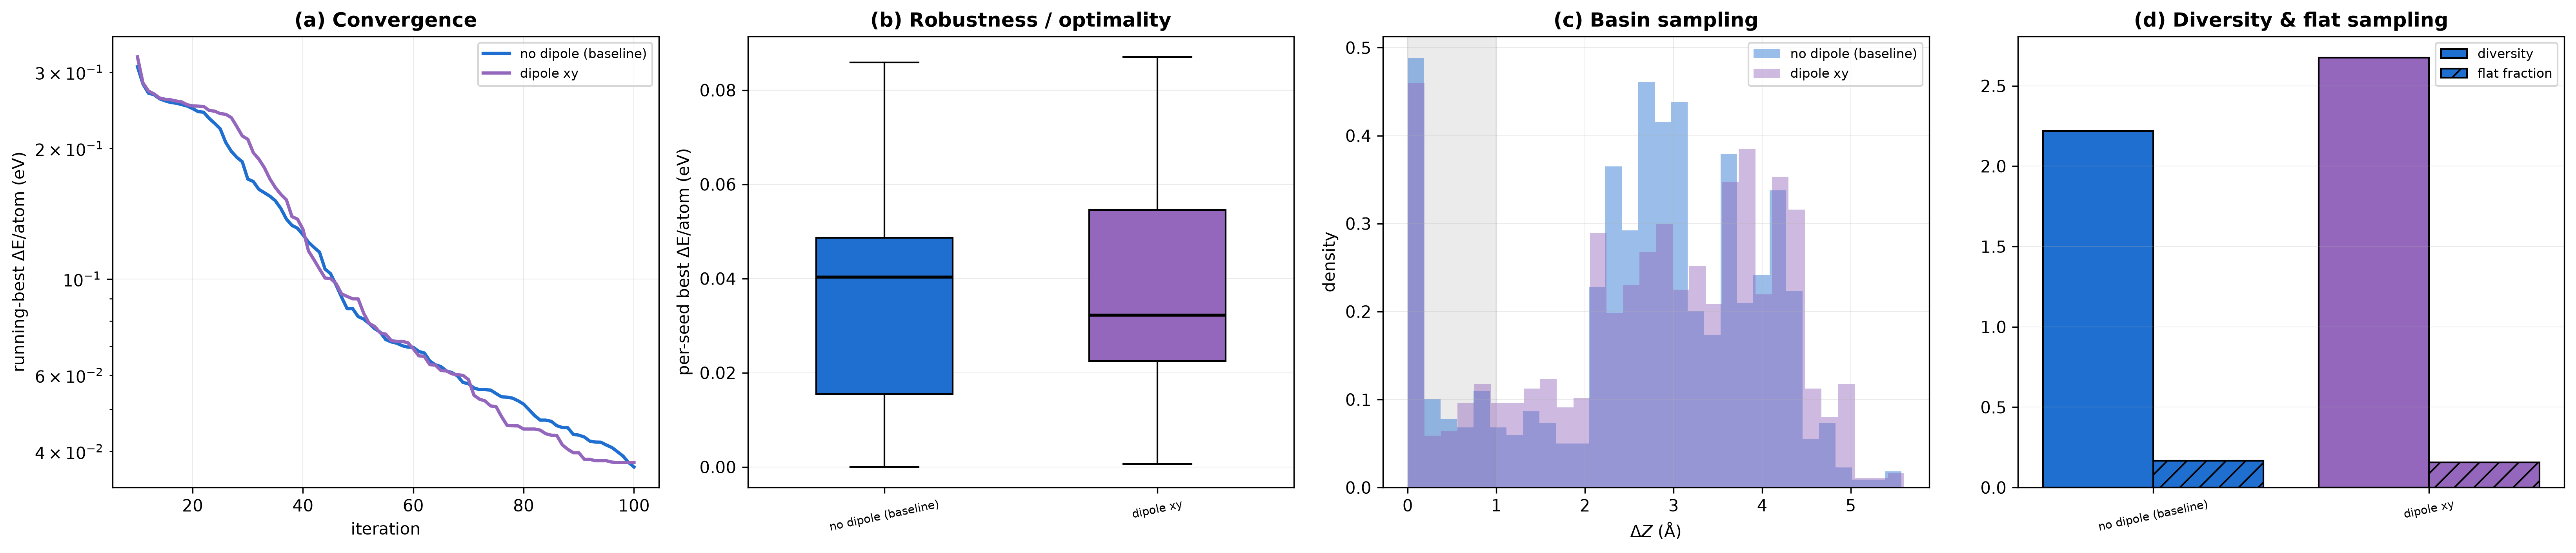
\includegraphics[width=\textwidth]{method_sensitivity_dipole.png}
\caption{\label{fig:S6}The same four panels for the dipole family.}
\end{figure}

\subsubsection{Reducing the rattle strength degrades the search by about 7$\times$} \emph{[SI-7]} Cutting
the two perturbation amplitudes roughly in half raises the per-seed best from 0.0368 to
0.2607 / 0.2558~\eVA---a factor of 7.1 and 7.0---and the flat-basin fraction collapses from
0.165 to 0.023 / 0.017. Reducing the perturbation is therefore not a cheaper equivalent of
the baseline: the rattle is what makes the search escape the initial region and reach the low-energy
basin at all, and less of it leaves the search sampling almost exclusively the island side. The
direction is not in doubt: every arm of the sweep is worse than the baseline, and the flat basin is
under-sampled by an order of magnitude in the flat fraction.

\subsubsection{The kappa parameter changes nothing measurable} \emph{[SI-5]} All four settings land within
0.0321--0.0395~\eVA---a total span of 0.0074~\eVA, far inside the standard deviations
(0.019--0.026)---so the method's conclusions are robust to the acquisition parameter, and in
particular no value of $\kappa$ can be identified as better than another from these runs.
There is a small, monotone trend in the flat-basin fraction---0.182, 0.165, 0.149 and 0.132 for
$\kappa = 1, 2, 3$ and 4---i.e.\ more exploration relative to exploitation samples slightly less of
the flat basin, but the effect is within the same order as the seed-to-seed spread.

\subsubsection{The dipole correction does not change the outcome} \emph{[SI-6]} The per-seed best moves
from 0.03683 $\pm$ 0.02575 to 0.03770 $\pm$ 0.02436~\eVA, a difference of 0.0009~\eVA---an order of
magnitude smaller than the standard deviation.

\section{The result does not depend on the search budget}
\label{sec:S4}

The main text reports the Fe/MgO model at a 100-iteration budget. To test whether the
\emph{comparison} the paper makes---the island being the ground state and the flat basin sitting
above it---survives a longer search, the same calculation was run to 200, 400 and 600
iterations: the run script is identical to the main-text one except for the number of iterations, and
the reference layer, the two perturbation generators and the acquisition parameter are unchanged. 6,
7 and 4 searches completed at 200, 400 and 600 iterations respectively.

\subsubsection{Method} The primary evidence is a per-run truncation: each search is cut at a
budget $k$ (100, then its own full budget) and the flat/island quantities recomputed, so the
100-iteration and full-budget numbers come from the \emph{same trajectory} and need no cross-run
normalisation. The flat/island split is $\dZ \le 1.0$~\AA{} and only iterations $\ge 10$ are used, as
in the main text. Each arm is tested against its own budget, and searches that stopped early are
excluded.

\begin{table}[t]
\small
\caption{\label{tab:S4}Flat-basin minimum $\Delta E/N$ (\eVA), pooled per arm at each budget (the
main-text definition: relative to the arm's own global minimum). The main-text model is the
100-iteration reference.}
\begin{tabular*}{\textwidth}{@{\extracolsep{\fill}}lccccc}
\toprule
Budget & completed searches & $k = 100$ & $k = 200$ & $k = 400$ & $k = 600$ \\
\midrule
200 iterations & 6 & 0.1901 & 0.1901 & --- & --- \\
400 iterations & 7 & 0.1624 & 0.1645 & 0.1662 & --- \\
600 iterations & 4 & 0.1807 & 0.1932 & 0.1966 & 0.1978 \\
main text (13 searches, 100 it) & 13 & \textbf{0.1888} & & & \\
\bottomrule
\end{tabular*}
\end{table}

\begin{figure}[t]
\centering
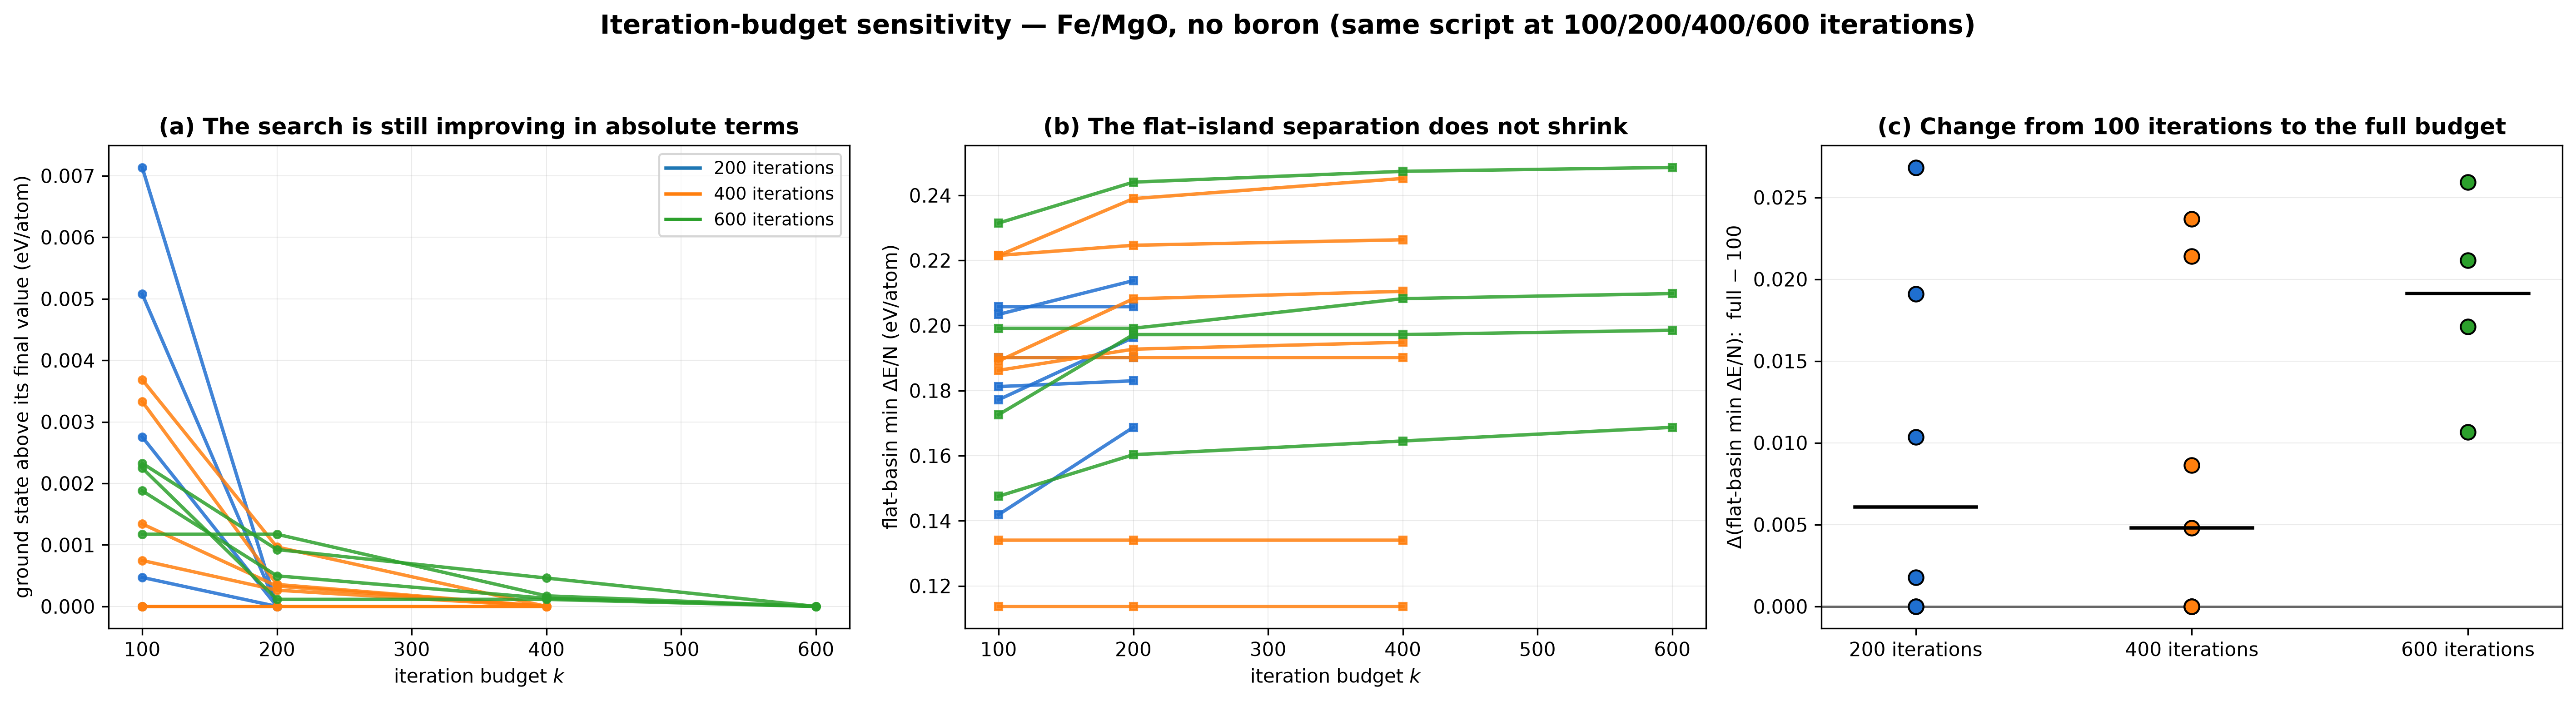
\includegraphics[width=\textwidth]{iteration_budget.png}
\caption{\label{fig:S7}(a) the absolute ground-state energy of each search against the budget,
showing that the search is still improving in absolute terms; (b) the flat--island separation of each
search against the budget, showing that it does not shrink; (c) the per-search change in the
flat-basin minimum from 100 iterations to the full budget.}
\end{figure}

\subsubsection{The island remains the ground state at every budget} In all 17 searches the lowest-energy
structure is an island at both the 100-iteration cut and the full budget. \emph{(MT-1)}

\subsubsection{The flat--island separation does not shrink with a longer search} Per run, the separation is
unchanged in 5 of the 17 searches and larger in the other 12---it never decreases---by a median of
+0.0104~\eVA (range 0 to +0.0268). Pooled per arm it rises from 0.1901 to 0.1901
(200 iterations), 0.1624 to 0.1662 (400) and 0.1807 to 0.1978~\eVA{} (600). A longer search therefore
does not bring the flat basin closer to the ground state; if anything it leaves it relatively higher.
\emph{(SI-9)}

The flat basin is a smaller fraction of the sampled set at longer budgets (0.165 at 100
iterations falling to 0.05--0.11 at 600). Longer searches keep finding better islands, so the flat
basin occupies a smaller share of the sampled structures.

\subsubsection{Cross-check} The 13 main-text searches, read through this analysis, reproduce the pooled
flat-basin minimum of 0.1888~\eVA{} exactly, so the two analyses agree on the reference value.

\section{The result does not depend on which phase sets the in-plane lattice}
\label{sec:S5}

The main-text model takes the Fe lattice constant for the simulation cell, so the substrate
carries the in-plane mismatch (compressed 3.6\,\% against its bulk value) and the film is
unstrained---the inverse of the experimental stack, where bulk MgO imposes its lattice on a thin
film. To test whether the structural result depends on this choice, the cell is swept from
Fe-matched to MgO-matched, $a = a_\mathrm{Fe} + f\cdot(a_\mathrm{MgO}/\sqrt{2} - a_\mathrm{Fe})$,
with both the film and the substrate built on that cell. The two endpoints are the
experimental lattice constants of the two bulk phases: bcc $\alpha$-Fe, $a = 2.866$~\AA{}
\cite{pietrokowsky1966}, and rocksalt MgO, $a = 4.2112$~\AA{} \cite{swanson1953} (4.212~\AA{} as used
in the inputs). At $f = 0.25$ the substrate is compressed 2.83\,\% and the film stretched 0.98\,\%;
at $f = 0.75$, $-0.94$\,\% and $+2.94$\,\%; at $f = 1.00$ the substrate sits at the experimental MgO
lattice constant and the film is stretched 3.92\,\%---the convention of the experimental stack. 10,
10 and 5 searches completed at $f = 0.25$, 0.75 and 1.00. The paper's own Fe/MgO model (13 searches,
cell $= a_\mathrm{Fe}$) is the Fe-matched reference; it uses the \emph{computed} Fe lattice constant
(2.87019~\AA) rather than the experimental 2.866~\AA, so the sweep's $f = 0$ endpoint is a reference,
not identical to the main-text model.

\begin{table}[t]
\scriptsize
\caption{\label{tab:S5}The constraint, the strains it puts on each phase, and the flat-basin minimum
(pooled, relative to each arm's own global minimum).}
\begin{tabular*}{\textwidth}{@{\extracolsep{\fill}}ccccccc}
\toprule
$f$ & cell $a$ (\AA) & substrate strain & film strain & searches & flat-basin min $\Delta E/N$ (\eVA) & island ground state \\
\midrule
0 (main text) & 2.87019 & $-3.63$\,\% & $0.00$\,\% & 13 & \textbf{0.1888} & yes \\
0.25 & 2.89408 & $-2.83$\,\% & $+0.98$\,\% & 10 & 0.1932 & yes \\
0.75 & 2.95025 & $-0.94$\,\% & $+2.94$\,\% & 10 & 0.1982 & yes \\
1.00 & 2.97833 & $0.00$\,\% & $+3.92$\,\% & 5 & 0.1907 & yes \\
\bottomrule
\end{tabular*}
\end{table}

\begin{figure}[t]
\centering
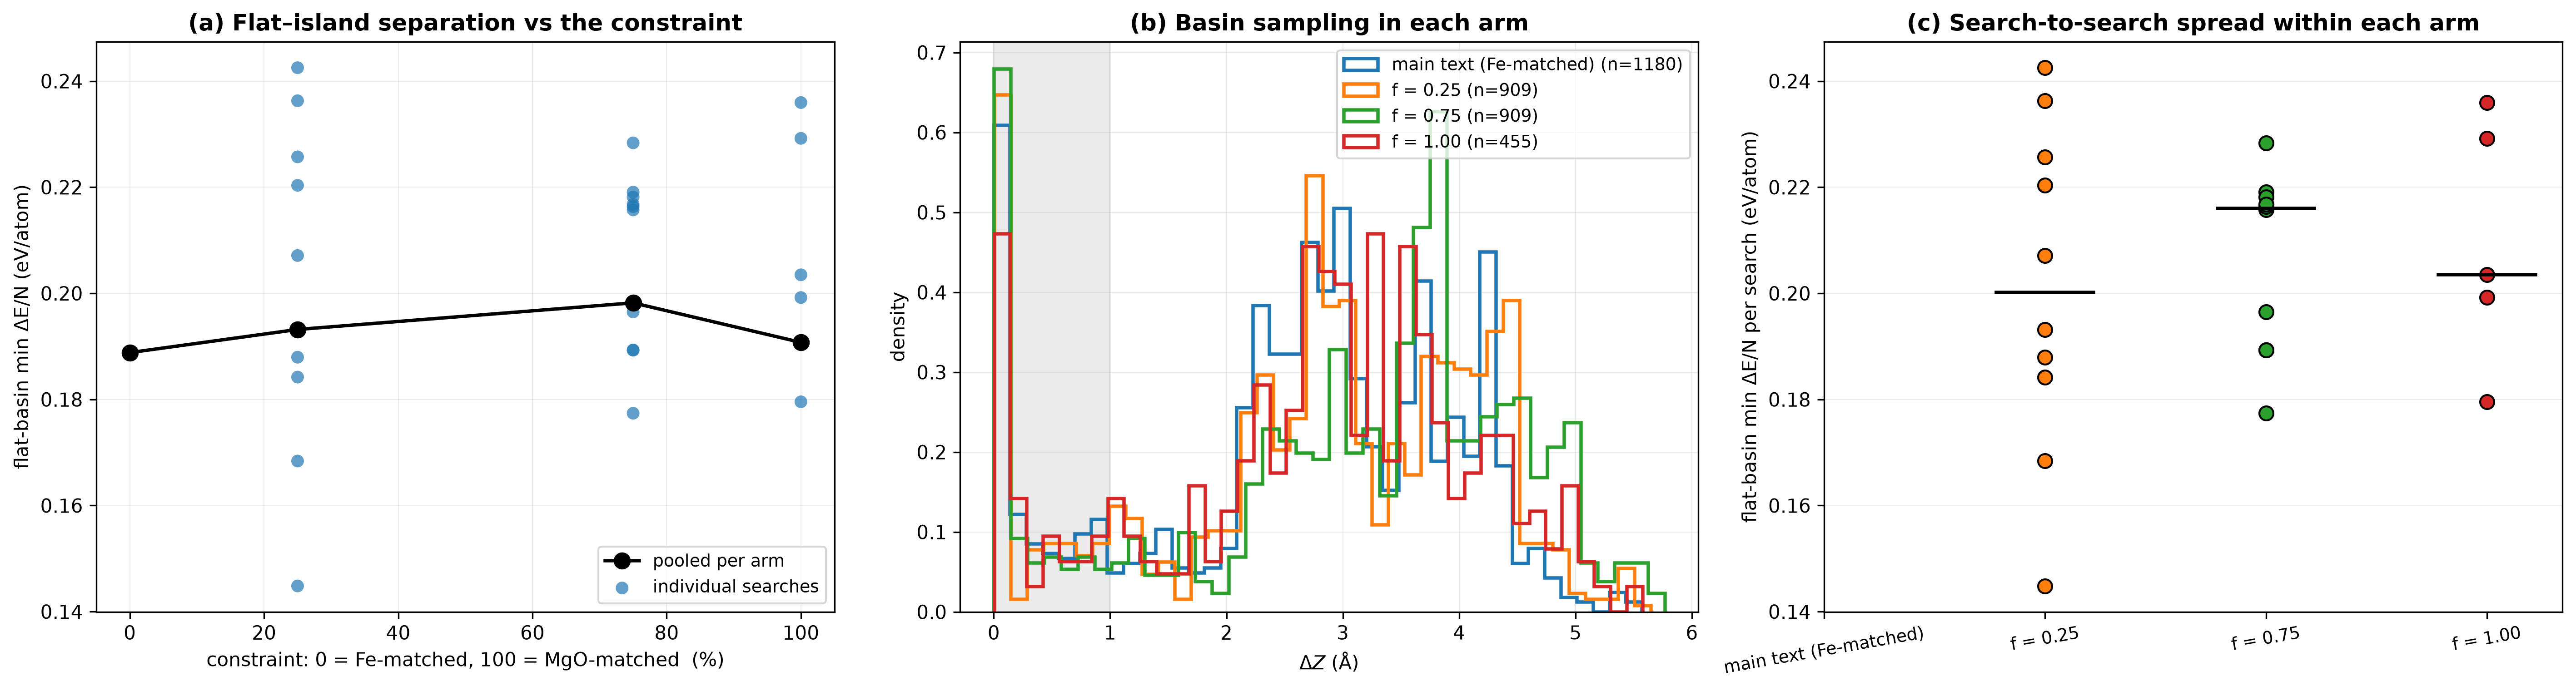
\includegraphics[width=\textwidth]{lattice_constraint.png}
\caption{\label{fig:S8}(a) the flat-basin minimum against the constraint, pooled per arm with the
individual searches overlaid; (b) the $\dZ$ distributions of each arm; (c) the search-to-search
spread within each arm.}
\end{figure}

\subsubsection{The island is the ground state under every constraint} In all 25 searches, at every value
of $f$, the lowest-energy structure is an island. \emph{(MT-1)}

\subsubsection{The flat-basin minimum is flat against the constraint} Pooled, it is 0.1932 ($f = 0.25$),
0.1982 ($f = 0.75$) and 0.1907~\eVA{} ($f = 1.00$), against 0.1888~\eVA{} for the Fe-matched
main-text model---a total spread of 0.0094~\eVA across the whole sweep. The
search-to-search scatter within an arm is 0.017--0.031~\eVA, i.e.\ 2--3$\times$ the entire sweep
effect, so no dependence on the constraint is resolvable. For scale, the constraint moves the
separation by about a quarter of the boron effect (0.040~\eVA). \emph{(SI-10)}

\subsubsection{The physically inverted strain case is therefore calculated for this model} The far end of
the sweep places the substrate at the experimental MgO lattice constant and stretches the
film---the convention of the experimental stack---and the result is unchanged.

\section{The inverted stack: a ground-state comparison (an MgO film on an Fe substrate)}
\label{sec:S6}

The main text studies Fe deposited on MgO, and its ground state is an island. Here we ask whether the
wetting of the deposited layer is symmetric---whether a film behaves the same way when it is
the oxide that is deposited. The comparison is made at the ground state of each stack: an
MgO film on an Fe substrate, against the Fe-on-MgO result of the main text. The inverted
stack uses the same system and scheme (Fe$_{25}$Mg$_{25}$O$_{25}$, 100 iterations, $\kappa = 2$, the
same two perturbation generators, cell at the experimental Fe lattice constant, 2.866~\AA).

\subsubsection{Method} The flatness is measured over the deposited film in each stack---Fe for
Fe-on-MgO, MgO (Mg $+$ O) for MgO-on-Fe---so the comparison is apples-to-apples on wetting. ($\dZ$
over Fe in the inverted stack would measure the substrate, which is flat by construction.) The ground
state is the lowest-energy structure of a stack, and the flat/island split is $\dZ \le 1.0$~\AA{} of
the deposited film. Only iterations $\ge 10$ are used, and only completed searches enter the
comparison.

\begin{table}[t]
\small
\caption{\label{tab:S6}The two stacks at their ground states.}
\begin{tabular*}{\textwidth}{@{\extracolsep{\fill}}lccc}
\toprule
Stack & Ground state & $\dZ$ of the deposited film & Flat film relative to the island \\
\midrule
Fe on MgO (main text) & island & 3.65~\AA & \textbf{+0.189~\eVA} above \\
\textbf{MgO on Fe (inverted)} & \textbf{flat film} & \textbf{0.39~\AA} & \textbf{$-0.016$~\eVA} below \\
\bottomrule
\end{tabular*}
\end{table}

\begin{figure}[t]
\centering
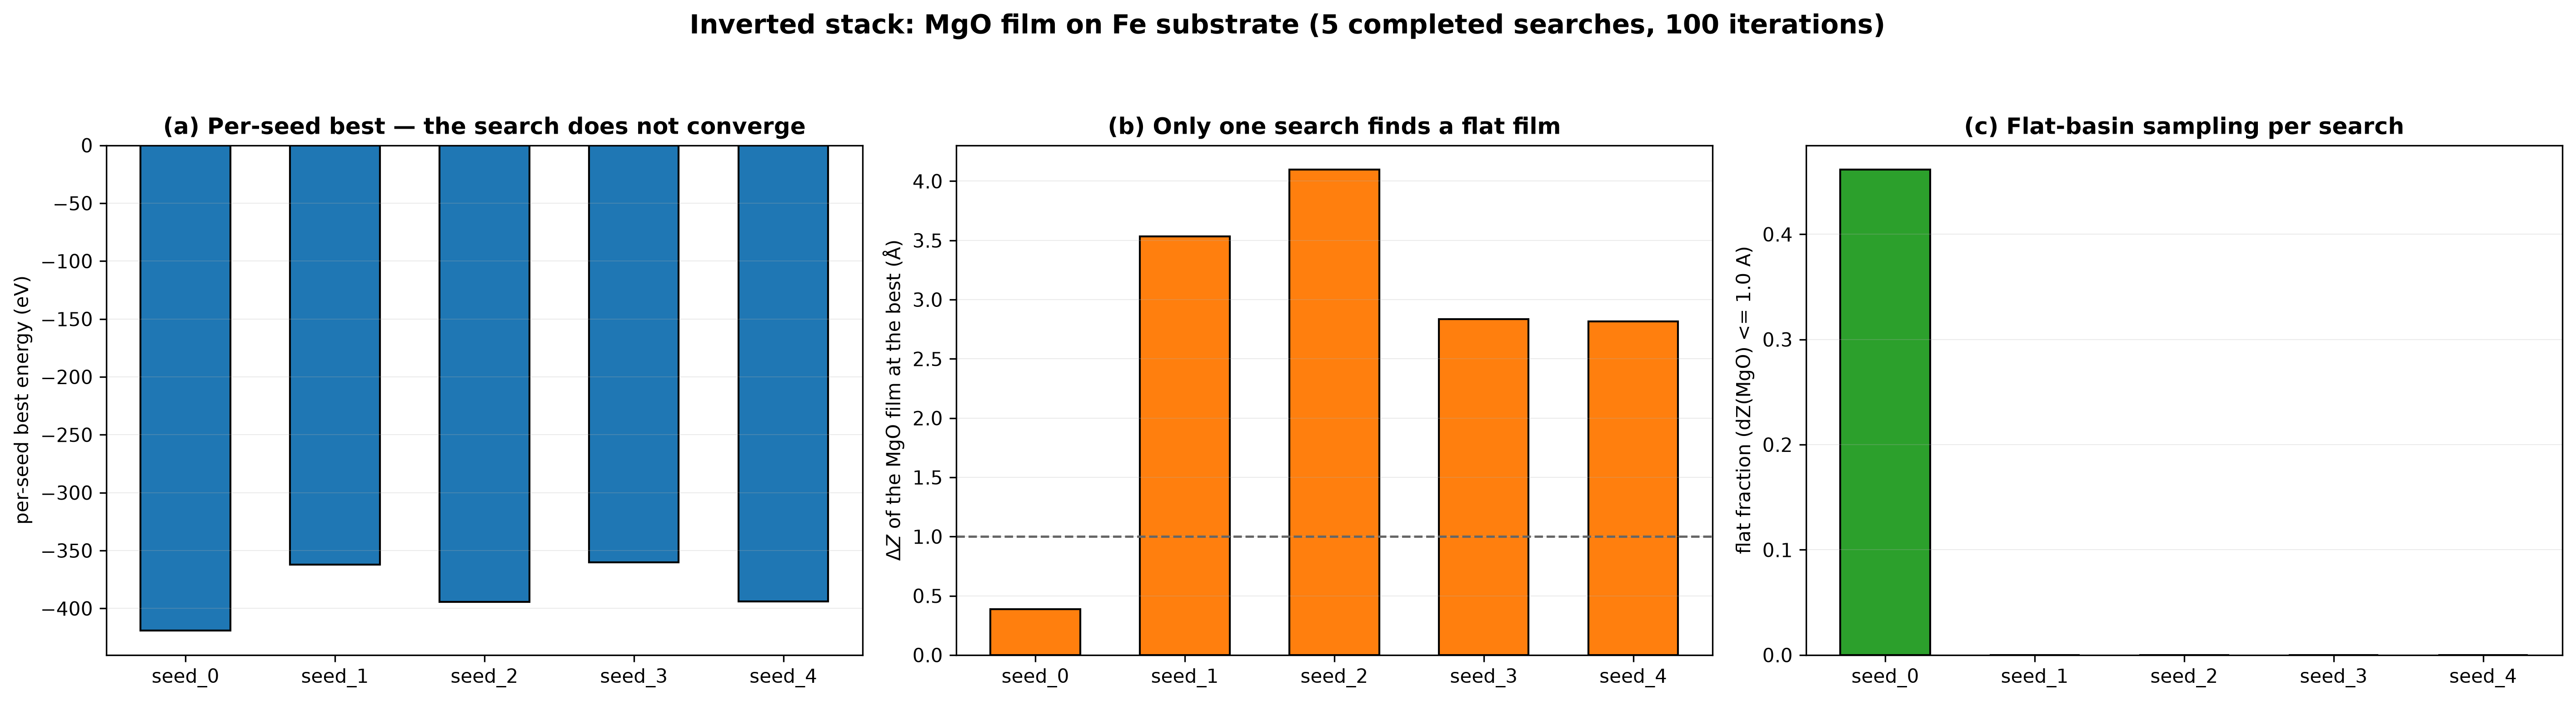
\includegraphics[width=\textwidth]{mgo_on_fe.png}
\caption{\label{fig:S9}(a) $\dZ$ of the deposited film at the ground state of each stack, against
the 1.0~\AA{} flat/island threshold; (b) where the flat film lies relative to the island for each
stack---positive means the island is the ground state, negative means the flat film is.}
\end{figure}

\subsubsection{The ground state of the inverted stack is a flat MgO film---the opposite of Fe-on-MgO} On
the inverted stack the lowest structure found is a flat MgO film ($\dZ = 0.39$~\AA), and the
flat film is 0.016~\eVA{} below the corresponding island. For Fe-on-MgO the ordering is the
reverse: the island is the ground state ($\dZ = 3.65$~\AA), and the flat film sits
0.189~\eVA{} above it. The sign of the wetting preference therefore inverts between the two
stacks---the layer that is deposited keeps its flat, wetting configuration when it is the oxide, and
breaks up into an island when it is the metal. \emph{(SI-11)}

\bibliographystyle{unsrtnat}
\bibliography{references}

\end{document}
